\documentclass{article}
\usepackage{enumitem}
\usepackage{listings}
\usepackage{amsfonts}
\usepackage{latexsym}
\usepackage{fullpage}
\usepackage{graphicx}
\usepackage{paralist}
\usepackage{tikz-timing}

\lstdefinelanguage{VHDL}{
  morekeywords={
    library,use,all,ENTITY,IS,PORT,IN,OUT,end,architecture,of,
    begin,and, ARCHITECTURE, IF, THEN, SIGNAL,END, PROCESS
  },
  morecomment=[l]--
}

\usepackage{xcolor}
\colorlet{keyword}{blue!100!black!80}
\colorlet{comment}{green!90!black!90}
\lstdefinestyle{vhdl}{
  language     = VHDL,
  basicstyle   = \ttfamily\scriptsize,
  keywordstyle = \color{keyword}\bfseries\ttfamily,
  commentstyle = \color{comment}\ttfamily,	
  tabsize=1
}

\renewcommand{\lstlistingname}{Code}

% Default margins are too wide all the way around. I reset them here
\setlength{\topmargin}{-.5in}
\setlength{\textheight}{9in}
\setlength{\oddsidemargin}{.125in}
\setlength{\textwidth}{6.25in}


%\let\oldenumerate\enumerate
%\renewcommand{\enumerate}{
  %\oldenumerate
  %\setlength{\itemsep}{1pt}
  %\setlength{\parskip}{0pt}
  %\setlength{\parsep}{0pt}
%}


\begin{document}
\title{Organization of Digital Computer Lab \\ EECS112L/CSE 132L}
\author{\textbf{Assignment 1 }\\ \textbf{Working with CAD tools} \\ \\
Student name: \\ Mario Ruiz \\Student ID: \\46301389 \\ \\ 
EECS Department\\ Henry Samueli School of Engineering \\ University of California, Irvine \\ \\
{January, 10, 2016}} 


\date{}
\maketitle


\section{What you've learned}
	I learned how to use the MentorGraphics Questasim toolset through the UCI Linux servers such as zuma.eecs.uci.edu in order to simulate and test VHDL code. We can also simulate and test our VHDL code using the Cadence Incisive toolset, however we need to use the UCI sun SPARC servers because the Linux servers don't support the Cadence toolset. 
	
	\section{MentorGraphics QuestaSim toolset}
 
	\subsection{Description}
		First we load the setup.csh and pre\_compile.csh files into the command prompt.\\
	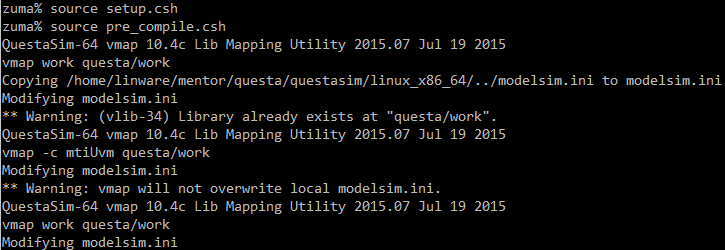
\includegraphics[width=0.45\textwidth]{mentor1.png}\\\\
		Next we compile the VHDL file for the alu.\\
	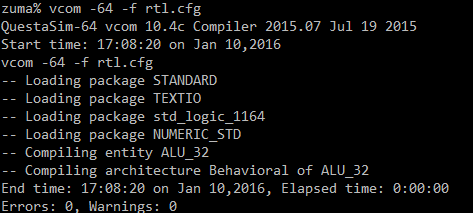
\includegraphics[width=0.45\textwidth]{mentor2.png}\\\\
		Then we compile the System Verilog file for the test bench.\\
	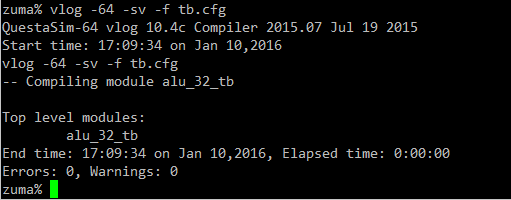
\includegraphics[width=0.45\textwidth]{mentor3.png}\\\\
		Then we optimize the VHDL design for the alu.\\
	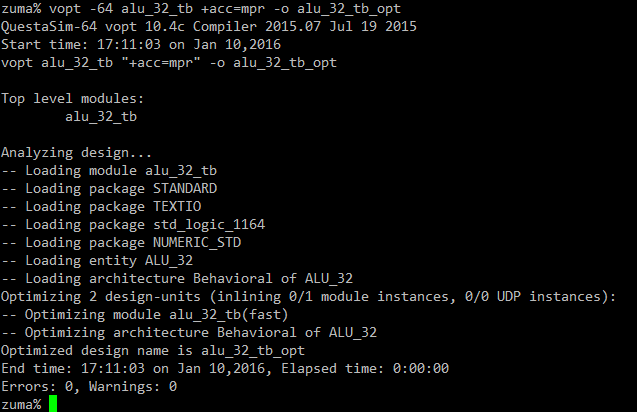
\includegraphics[width=0.45\textwidth]{mentor4.png}\\\\
		Finally, we simulate the alu using the testbench.\\
	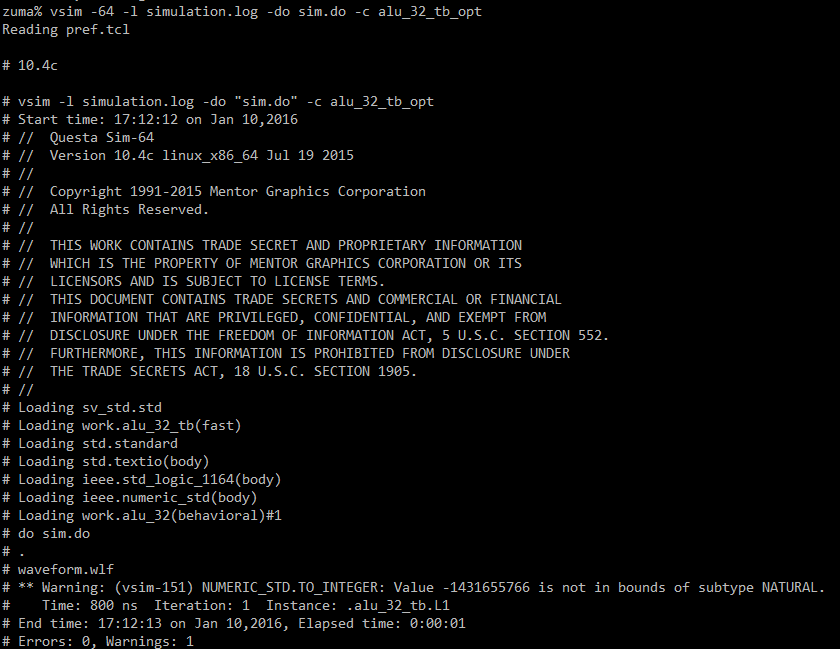
\includegraphics[width=0.45\textwidth]{mentor5.png}
	
	\subsection{Simulation waveform}

	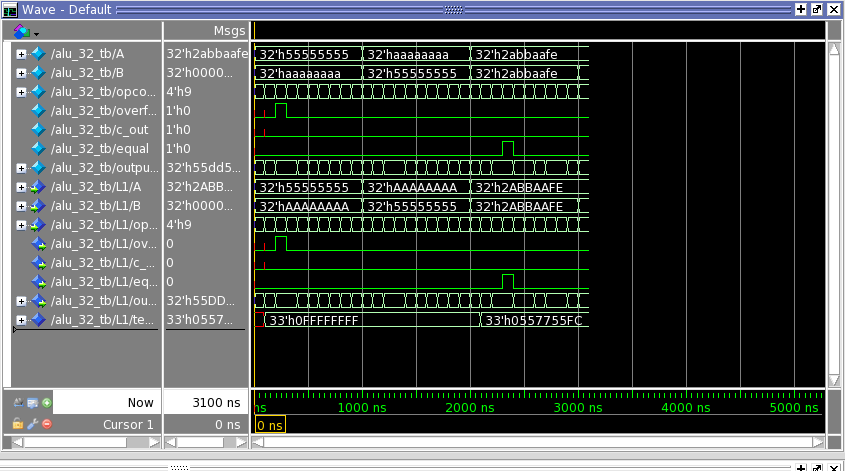
\includegraphics[width=0.6\textwidth]{Questasim_waveform.png}

\section{Cadence Incisive toolset}

	\subsection{Description}
		First, compile the vhdl code for the orgate and the tb.\\
	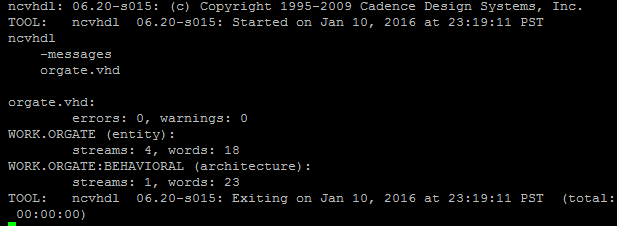
\includegraphics[width=0.5\textwidth]{cadence1.png}\\\\
		Next elaborate and run the simulation in order for it to make the appropriate waveforms.\\
	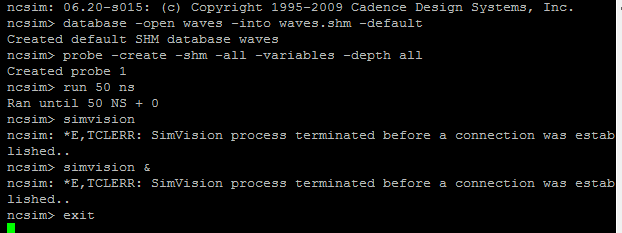
\includegraphics[width=0.5\textwidth]{cadence2.png}

	\subsection{Simulation waveform}

	\bfseries{Simulation Waveform is as follows:} \\ \\

	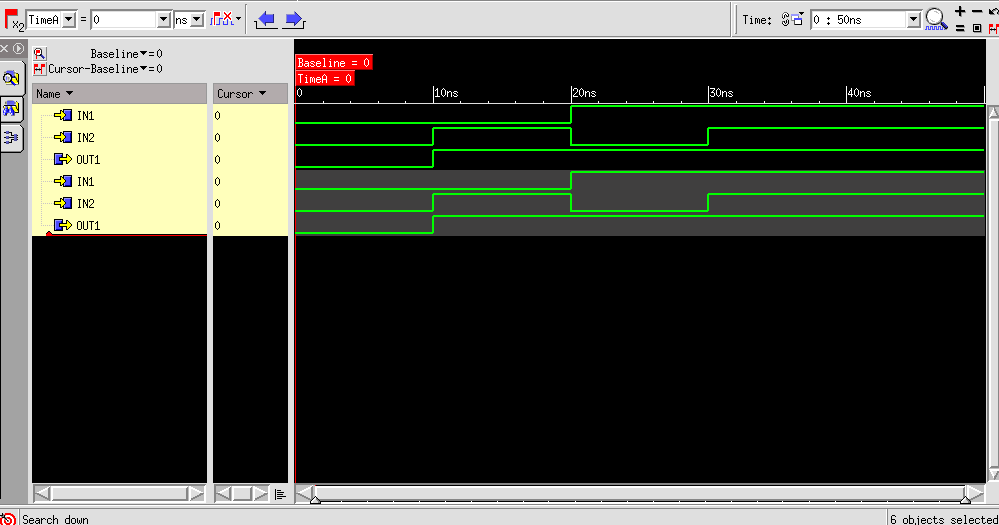
\includegraphics[width=0.6\textwidth]{Cadence_waveform.png}

\section{Conclusion}

	I would prefer to use the MentorGraphics Questasim toolset for the 112L course because the Cadence Incisive toolset needed a lot more steps to work properly. For example we need to set up a project folder with many other file for each new project. Also there was more work needed in order to view the waveforms in Cadence. On the other hand, the MentorGraphics toolset did not need any new files created other then the actual files for the assignment. Also the waveform was easily viewed compared to the Cadence toolset. Overall my experience with the MentorGraphics toolset was a lot less tedious.  


\end{document}
